%!TEX program = xelatex
\documentclass[dvipsnames, svgnames,a4paper,11pt]{article}
% ----------------------------------------------------
%   中山大学物理与天文学院本科实验报告模板
%   作者:Huanyu Shi,2019级
%   知乎:https://www.zhihu.com/people/za-ran-zhu-fu-liu-xing
%   Github:https://github.com/Huanyu-Shi/SYSU-SPA-Labreport-Template
%   Last update : 2023.4.10
% ----------------------------------------------------

% ----------------------------------------------------- 
%	加边框的命令
%	参考:https://tex.stackexchange.com/questions/531559/how-to-add-the-page-border-for-first-two-pages-in-latex
\usepackage{tikz}
\usetikzlibrary{calc}
\usepackage{eso-pic}
\AddToShipoutPictureBG{%
\begin{tikzpicture}[overlay,remember picture]
\draw[line width=0.6pt] % 边框粗细
    ($ (current page.north west) + (0.6cm,-0.6cm) $)
    rectangle
    ($ (current page.south east) + (-0.6cm,0.6cm) $); % 边框位置
\end{tikzpicture}}


\usepackage{xcolor}
\definecolor{c1}{HTML}{2752C9} % 目录颜色
\definecolor{c2}{RGB}{190,20,83} % 引用颜色

\usepackage{ctex}
\usepackage[top=28mm,bottom=28mm,left=15mm,right=15mm]{geometry}
\usepackage{hyperref} 
\hypersetup{
	colorlinks,
	linktoc = section, % 超链接位置,选项有section, page, all
	linkcolor = c1, % linkcolor 目录颜色
	citecolor = c1  % citecolor 引用颜色
}
\usepackage{amsmath,enumerate,multirow,float}
\usepackage{tabularx}
\usepackage{tabu}
\usepackage{subfig}
\usepackage{fancyhdr}
\usepackage{graphicx}
\usepackage{wrapfig}  
\usepackage{physics}
\usepackage{appendix}
\usepackage{amsfonts}

%
\usepackage{tcolorbox}
\tcbuselibrary{skins,breakable}
\newtcolorbox{tbox}[2][]{
    colframe=black!70!,
    breakable,
    enhanced,
	boxrule =0.5pt,
    title = {#2},
    fonttitle = \large\kaishu\bfseries,
	drop fuzzy shadow,
    #1
}
\newtcolorbox[auto counter,number within=section]{question}[1][]{
  top=2pt,bottom=2pt,arc=1mm,
  boxrule=0.5pt,
%   frame hidden,
  breakable,
  enhanced, %跨页后不会显示下边框
  coltitle=c1!80!gray,
  colframe=c1,
  colback=c1!3!white,
  drop fuzzy shadow,
  title={思考题~\thetcbcounter:\quad},
  fonttitle=\bfseries,
  attach title to upper,
  #1
}
\newcommand{\setLhead}[1]{%
  \lhead{{\color{gray}\kaishu #1}} % 定义新的命令,设置右边页眉的内容
}
\newcommand{\setRhead}[1]{%
  \rhead{{\color{gray}\kaishu #1}} % 定义新的命令,设置右边页眉的内容
}
% ---------------------------------------------------------------------
%	利用cleveref改变引用格式,\cref是引用命令
\usepackage{cleveref}
\crefformat{figure}{#2{\textcolor{c2}{图 #1}}#3} % 图片的引用格式
\crefformat{equation}{#2{(\textcolor{c2}{#1})}#3} % 公式的引用格式
\crefformat{table}{#2{\textcolor{c2}{表 #1}}#3} % 表格的引用格式


% ---------------------------------------------------------------------
%	页眉页脚设置
\fancypagestyle{plain}{\pagestyle{fancy}}
\pagestyle{fancy}
\setLhead{中山大学物理与天文学院基础物理实验预习报告}
%\lhead{\kaishu 中山大学物理与天文学院物理实验\uppercase\expandafter{\romannumeral3}} % 左边页眉,学院 + 课程
%\rhead{{\color{gray}\kaishu Template 实验报告模板}} % 右边页眉,实验报告标题
\setRhead{实验1\hspace{1pt}冰的熔化热测量}
\cfoot{\thepage} % 页脚,中间添加页码


% ---------------------------------------------------------------------
%	对目录、章节标题的设置
\renewcommand{\contentsname}{\centerline{\huge 目录}}
\usepackage{titlesec}
\usepackage{titletoc}
% \titleformat{章节}[形状]{格式}{标题序号}{序号与标题间距}{标题前命令}[标题后命令]
\titleformat{\section}{\centering\LARGE\songti}{}{1em}{}

% ---------------------------------------------------------------------
%   listing代码环境设置
\usepackage{listings}
\lstloadlanguages{python}
\lstdefinestyle{pythonstyle}{
backgroundcolor=\color{gray!5},
language=python,
frameround=tftt,
frame=shadowbox, 
keepspaces=true,
breaklines,
columns=spaceflexible,                   
basicstyle=\ttfamily\small, % 基本文本设置,字体为teletype,大小为scriptsize
keywordstyle=[1]\color{c1}\bfseries, 
keywordstyle=[2]\color{Red!70!black},   
stringstyle=\color{Purple},       
showstringspaces=false,
commentstyle=\ttfamily\scriptsize\color{green!40!black},%注释文本设置,字体为sf,大小为smaller
tabsize=2,
morekeywords={as},
morekeywords=[2]{np, plt, sp},
numbers=left, % 代码行数
numberstyle=\it\tiny\color{gray}, % 代码行数的数字字体设置
stepnumber=1,
rulesepcolor=\color{gray!30!white}
}




% ---------------------------------------------------------------------
%	其他设置
\def\degree{${}^{\circ}$} % 角度
\graphicspath{{./images/}} % 插入图片的相对路径
\allowdisplaybreaks[4]  %允许公式跨页 % 导入模板的相关设置
\usepackage{lipsum}
\usepackage{indentfirst}
\usepackage{pdfpages}
\usepackage{multirow}
\usepackage{subfig}
\usepackage{graphicx}
\usepackage{float} 
\usepackage{booktabs}
\usepackage{enumerate}
\usepackage{makecell} 
\renewcommand{\d}{\mathrm{d}}
\newcommand{\upcite}[1]{\textsuperscript{\textsuperscript{\cite{#1}}}}


%---------------------------------------------------------------------
%	正文
%---------------------------------------------------------------------
\newcommand{\exname}{光学像差I}%实验名称
\setRhead{\exname}
\begin{document}


\begin{table}
	\renewcommand\arraystretch{1.7}
	\begin{tabularx}{\textwidth}{
		|X|X|X|X
		|X|X|}
	\hline
	\multicolumn{2}{|c|}{预习报告}&\multicolumn{2}{|c|}{实验记录}&\multicolumn{2}{|c|}{总成绩}\\
	\hline
	 \hspace{0.625cm}30& & \hspace{0.625cm}50  & &  \hspace{0.625cm}80 & \\
	\hline
	\end{tabularx}
\end{table}


\begin{table}
	\renewcommand\arraystretch{1.7}
	\begin{tabularx}{\textwidth}{|X|X|X|X|}
	\hline
	专业:& 物理学类 &年级:&2023级 \\
	\hline
	姓名:& 姚昊廷  & 学号:&22322091\\
	\hline
	日期:&2025.3.18& 教师签名:& \\
	\hline
	\end{tabularx}
\end{table}

\begin{center}
	\LARGE \exname
\end{center}

\textbf{【实验报告注意事项】}
\begin{enumerate}
	\item 实验报告由三部分组成:
	\begin{enumerate}
		\item 预习报告:阅读\underline{\textbf{实验讲义}},弄清实验原理,了解实验需要测量的物理量,完成预习思考题。将预习报告带到实验室并在开始实验前由实验教师或助教检查。预习成绩低于10分(共20分)者不能做实验。
	    \item 实验记录与分析:认真、客观记录实验条件、实验过程中的现象以及数据。实验记录请用珠笔或者钢笔书写并签名(\textcolor{red}{\textbf{用铅笔记录的被认为无效}})。\textcolor{red}{\textbf{保持原始记录,包括写错删除部分。}}离开前请实验教师或助教检查记录并签名。
	\end{enumerate}
	\item 本实验报告可提前打印出来,当场记录分析完成交给带实验的老师,课后无需再提交。若当场完成不了,则请课后完成,再扫描并通过seelight提交。
	\item \textbf{【安全注意事项】}
    \begin{enumerate}
        \item 实验中避免激光器伤到眼睛
        \item 避免用手直接接触镜片的光学面
        \item 安装镜片时需在光学平台上尽量靠近台面的高度操作,以免失手跌落摔碎镜片
        \item 实验平台配件所用固定螺钉需拧紧,以免镜架晃动;但不可过紧,以免损坏
        \item 实验前需按仪器清单检查光学元件是否齐全,实验结束后按照顺序放回元件盒
    \end{enumerate}
\end{enumerate}

\clearpage
\tableofcontents
\clearpage

\setcounter{section}{0}
\section{\exname\ \textbf{预习报告}}
	
\subsection{实验目的}
\begin{enumerate}
	\item 了解七种几何像差产生的原理、基本规律;
	\item 了解各种像差对光学成像质量的影响;
	\item 掌握慧差、色差产生的原理及其测量表征;
	\item 掌握光学系统的基本调试方法;
\end{enumerate}
\subsection{仪器用具}
\begin{table}[H]
	\centering
	\renewcommand\arraystretch{1.6}
	% \setlength{\tabcolsep}{10mm}
	\scalebox{0.7}{
	\begin{tabular}{p{0.05\textwidth}|p{0.20\textwidth}|p{0.05\textwidth}|p{0.5\textwidth}}
	\hline
	编号& 仪器用具名称 & 数量 &  主要参数(型号,测量范围,测量精度等) \\
	\hline
	1&激光光源&1 &$\lambda$=632.6nm\\
	2&激光器夹持器&1 &3维调整\\
	3&显微物镜&1 &10$\times$/0.25\\
	4&针孔&1 &$\phi$100um或$\phi$50um\\
	5&五维调整机构&1 &装配显微物镜和针孔用\\
	6&衰减片1&1 &0.0001(衰减系数),装在镜框中\\
    7&衰减片2&1 &0.01(衰减系数),装在镜框中\\
    8&双凸透镜1&1 &焦距f=300mm,装在透镜/反射镜座中\\
    9&平凸透镜2&1 &焦距f=100mm,装在透镜/反射镜座中\\
    10&平凸透镜3&1 &焦距f=150mm,装在透镜/反射镜座中\\
    11&白屏&1 &SZ-13,一面白屏,一面带坐标纸\\
    12&成像相机&1 &大恒的MER-130-30UM或元启智能的REV-13AMU2C\\
    13&数据线&1 &图像采集数据线\\
    14&计算机&1 &台式或笔记本,安装有成像相机图像采集软件\\
    15&光学导轨&1 &长度1米,带刻度\\
    16&二维平移台&4&行程>10mm\\
    17&平移滑块&1 &\\
    18&支杆&3+5 &50mm长和75mm长\\
    19&磁性表座&4 &\\
    20&旋转调整台&1 &可调角度$>\pm 5^\circ$\\
    21&白光灯&1 &GY-6型,亮度可调,即溴钨灯\\
    22&滤光片1&1 &透光波长:435nm\\
    23&滤光片2&1 &透光波长:630nm\\
	\hline
\end{tabular}}
\end{table}


\subsection{原理概述}
\begin{enumerate}
	\item 色差\begin{enumerate}
		\item 原理:
		色差源于光学材料对不同波长(颜色)光的折射率差异(即色散现象)。
		\begin{enumerate}
			\item 折射率与波长的关系:光学材料的折射率随波长增大而减小(正常色散)。例如,蓝光(短波长)折射率较高,红光(长波长)折射率较低。
			\item 焦点位置偏移:\begin{enumerate}
				\item 轴向色差(纵向色差):不同波长的光通过透镜后,蓝光因折射率大,会聚在更靠近透镜的焦点;红光折射率小,焦点更远离透镜。这导致同一物体发出的光在光轴方向上形成多个焦点,成像模糊。
				\item 横向色差(倍率色差):不同波长的光在成像平面上的放大率不同。例如,红光可能比蓝光成像稍大,导致物体边缘出现彩色镶边(如紫边或红边)。
			\end{enumerate}
		\end{enumerate}
	\end{enumerate}
	\item 慧差
	\begin{enumerate}
		\item 原理:
		慧差是离轴点光源通过光学系统时,因透镜不同区域对光线的折射不对称导致的像差。
		\begin{enumerate}
			\item 离轴光线的折射差异:当光线从光轴外某点(离轴点)入射时,通过透镜不同环带区域(如边缘与中心)的光线折射角度不同。
			\begin{enumerate}
				\item 透镜边缘区域的入射角较大,折射后偏离理想成像点的程度更显著。
				\item 中心区域的折射较接近理想路径,但边缘区域的折射光线会形成偏离主光轴的聚焦点。
			\end{enumerate}
			\item 彗星状光斑的形成:\begin{enumerate}
				\item 离轴光线经透镜不同环带折射后,无法汇聚于同一点,而是沿主光线方向形成一系列逐渐扩散的焦点。
				\item 例如,透镜边缘的光线聚焦点离主光线更远,形成“彗尾”;中心区域光线形成“彗头”,最终成像为头部明亮、尾部渐暗的不对称光斑。
			\end{enumerate}
			\item 视场角的影响:慧差随视场角(光线与光轴的夹角)增大而加剧,在广角镜头或大孔径系统中尤为明显。
		\end{enumerate}
	\end{enumerate}
\end{enumerate}
色差本质是色散导致不同颜色光的传播路径分离。

慧差本质是离轴光线因透镜区域折射差异形成的非对称像差。
两者均破坏成像的清晰度和准确性,但其物理根源分别在于材料的波长依赖性和几何光学的不对称性。
\subsection{预习思考题}
\begin{question}
	慧差与孔径、视场的关系?
	\tcblower
	慧差的严重程度与光学系统的孔径(光束口径)和视场(光线离轴角度)密切相关,在实际光学系统中,慧差的综合影响可表示为:
	\begin{align*}
		\text{慧差}\propto (\text{孔径})^3\times(\text{视场角})^2
	\end{align*}
	透镜边缘区域的入射角较大,孔径越大,边缘光线与中心光线的折射差异越显著。慧差的幅度与孔径的三次方成正比(即与孔径直径的立方相关)。离轴光线偏离光轴越远,通过透镜不同区域的折射路径差异越大,导致成像点的不对称扩散更显著。
	慧差的幅度与视场角(光线与光轴的夹角)的平方成正比。
\end{question}

\begin{question}
	产生色差原因?列举几种消色差的方法
	\tcblower
	色差是由于光学材料的折射率随波长变化(色散效应)引起的像差,表现为不同颜色的光无法汇聚到同一焦点。
	消除方法主要有:
	\begin{enumerate}
		\item  复合透镜:组合两种不同色散特性的材料(如冕牌玻璃和火石玻璃),利用其相反的色散特性抵消色差。
		\item 使用特殊材料(如萤石、ED超低色散玻璃),其色散曲线更平缓,折射率对波长依赖性更低。
		\item 通过三片或更多透镜组合(使用三种不同色散材料),将红、绿、蓝三色光的焦点对齐,进一步消除二级光谱(残余色差)。
		\item 非球面表面可优化不同区域的光路,减少因球面曲率导致的色散累积效应。
		\item 缩小光圈(减小有效孔径),减少边缘光线的参与,降低色散差异的影响。
		\item 利用衍射光栅的色散特性与折射透镜的色散相反,抵消色差。
		\item 通过图像处理算法(如Adobe Lightroom、相机机内校正),识别并消除照片中的色差(如紫边修正)。
		\item 减少透镜表面的反射损失,抑制因多次反射引起的杂散光(间接缓解色差)。
	\end{enumerate}
\end{question}

\begin{question}
	针孔滤波的工作原理
	\tcblower
	针孔滤波是一种基于空间频率选择的光学滤波技术,其核心原理是通过物理小孔对光波的传播路径或空间频率成分进行限制,从而实现噪声抑制、分辨率提升或特定模式的提取。\\
	空间滤波:光波携带的信息包含不同方向(空间频率)的成分。针孔作为空间滤波器,通过限制光束的传播角度或截取特定区域的光场,选择性地允许某些空间频率通过,阻挡其他成分。\\
	物理限制:小孔的直径决定了允许通过的光波的最大空间频率(即截止频率),孔径越小,截止频率越低,高频成分被阻挡。
\end{question}
\clearpage
\setLhead{中山大学物理与天文学院基础物理实验记录}
\begin{table}
	\renewcommand\arraystretch{1.7}
	\centering
	\begin{tabularx}{\textwidth}{|X|X|X|X|}
	\hline
	专业:& 物理学类 &年级:& 2023级 \\
	\hline
	姓名: &姚昊廷& 学号:&22322091  \\
	\hline
	室温:&$22^\circ$C&实验地点:&A505  A4\\
	\hline
	学生签名:& & 评分: &\\
	\hline
	实验时间:& 2025.3.4& 教师签名:&\\
	\hline
	\end{tabularx}
\end{table}
\section{\exname\ \textbf{实验记录}}
\subsection{实验内容、步骤、结果}


\clearpage
\setLhead{中山大学物理与天文学院基础物理实验分析与讨论}
\begin{table}
	\renewcommand\arraystretch{1.7}
	\begin{tabularx}{\textwidth}{|X|X|X|X|}
	\hline
	专业:& 物理学 &年级:& 2023级\\
	\hline
	姓名: &姚昊廷& 学号:&22322091 \\
	\hline
    日期:&2025.3.4 &  &\\
	\hline
	评分:&&教师签名:&\\
	\hline
	\end{tabularx}
\end{table}

\section{\exname\ \textbf{分析与讨论}}
\subsection{分析与讨论}

\subsection{实验后思考题}


\clearpage
% ---------------------------------------------------------------------
%   参考文献
%   注:使用参考文献时应按照xelatex->bibtex->xelatex->xelatex顺序进行编译
%\phantomsection
%\addcontentsline{toc}{section}{参考文献}
%\bibliographystyle{unsrt}
%\bibliography{myref}
%\begin{thebibliography}{9}
%	\bibitem{ref1} 沈雨欣,翁存程,蒋丽钦.双棱镜干涉法准确测量钠光波长[J].大学物理实验,2023,36(03):40-43.DOI:10.14139/j.cnki.cn22-1228.2023.03.008.
%	\bibitem{ref2} 牟泉润,孙丽媛,杜月棋,等.基于干涉原理的光波长测量装置设计[J].大学物理实验,2021,34(06):80-83+89.DOI:10.14139/j.cnki.cn22-1228.2021.06.018.
%	\bibitem{ref3} 王仁洲,杨涛.一种用激光干涉测量光波波长的新方法[J].大学物理实验,2014,27(06):41-43.DOI:10.14139/j.cnki.cn22-1228.2014.06.014.
%\end{thebibliography}


%\clearpage
\appendix
\appendixpage
\addappheadtotoc
%\subsection*{相图代码}
%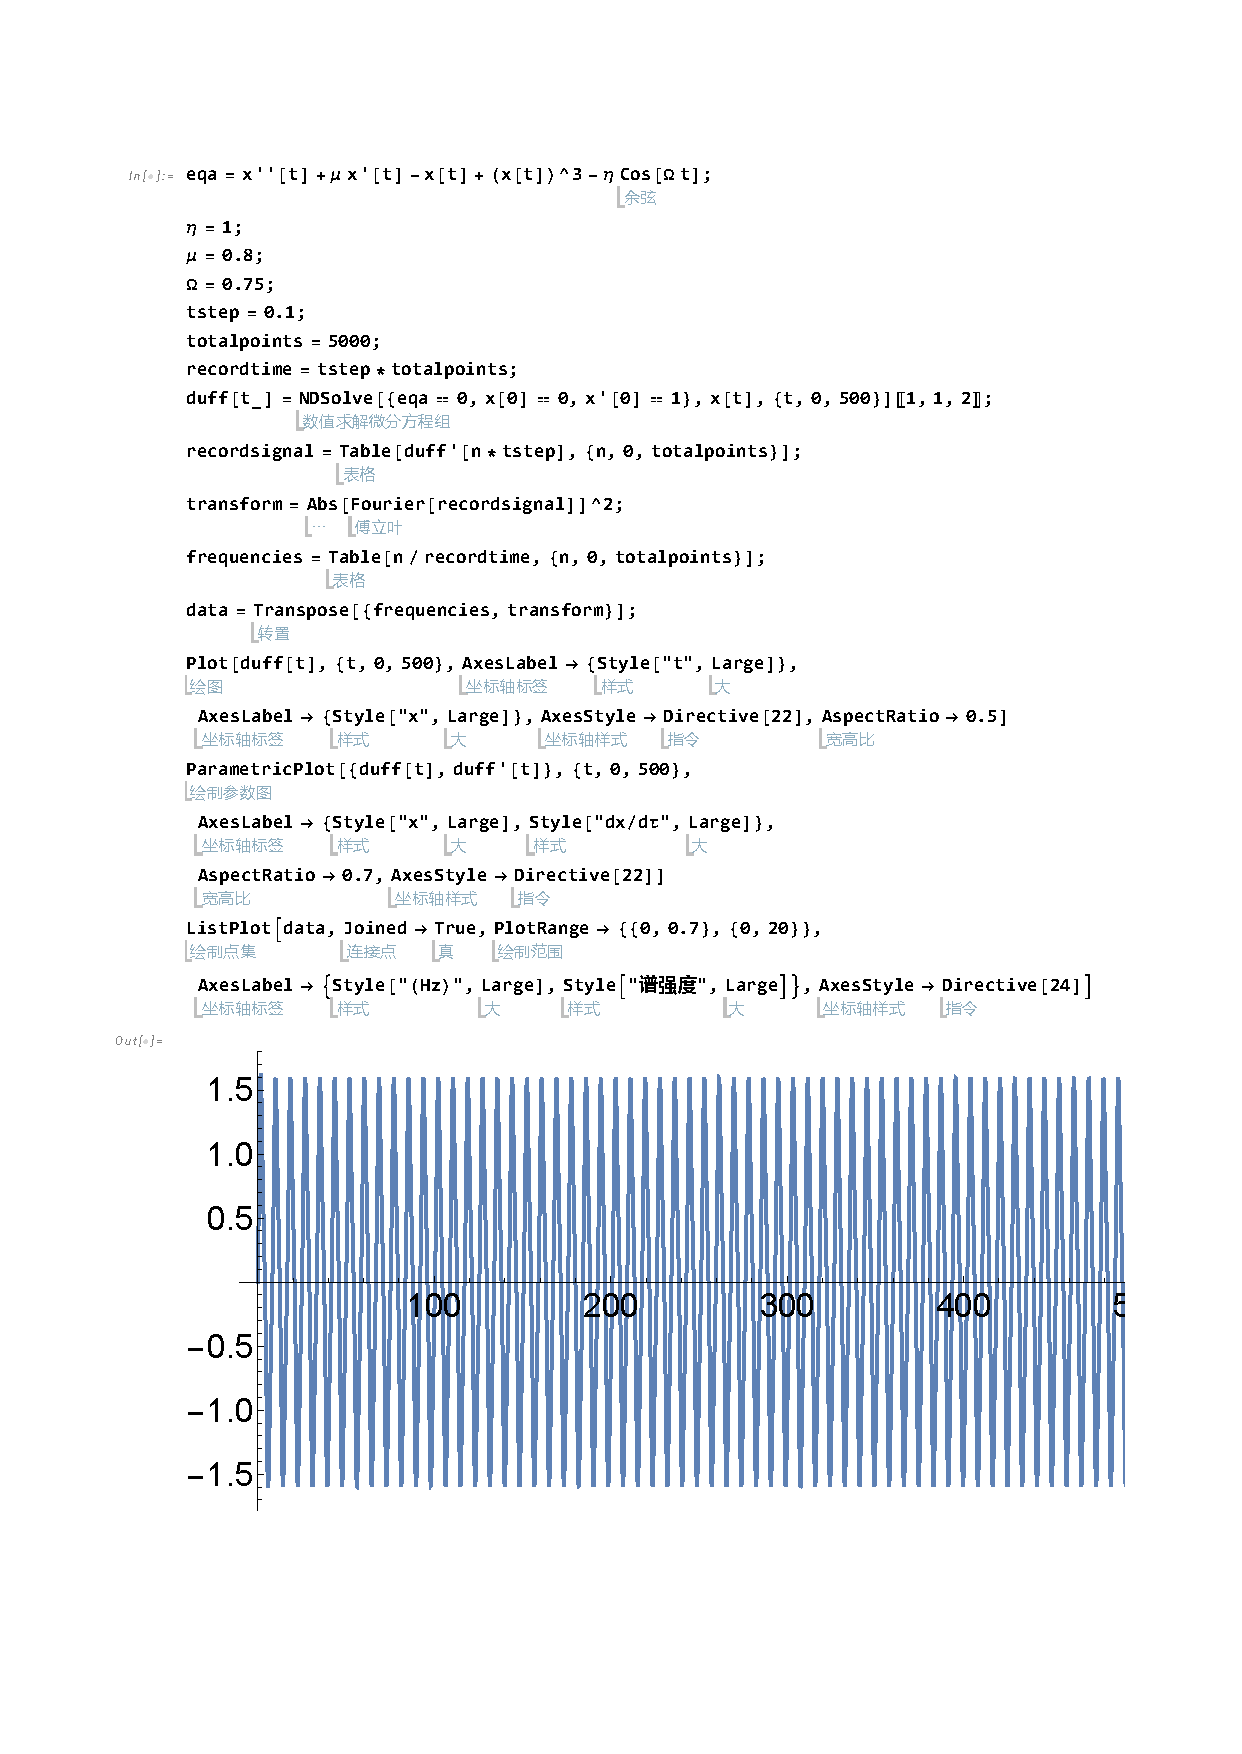
\includepdf[pages=-]{chaos.pdf}
%\subsection*{原件}
%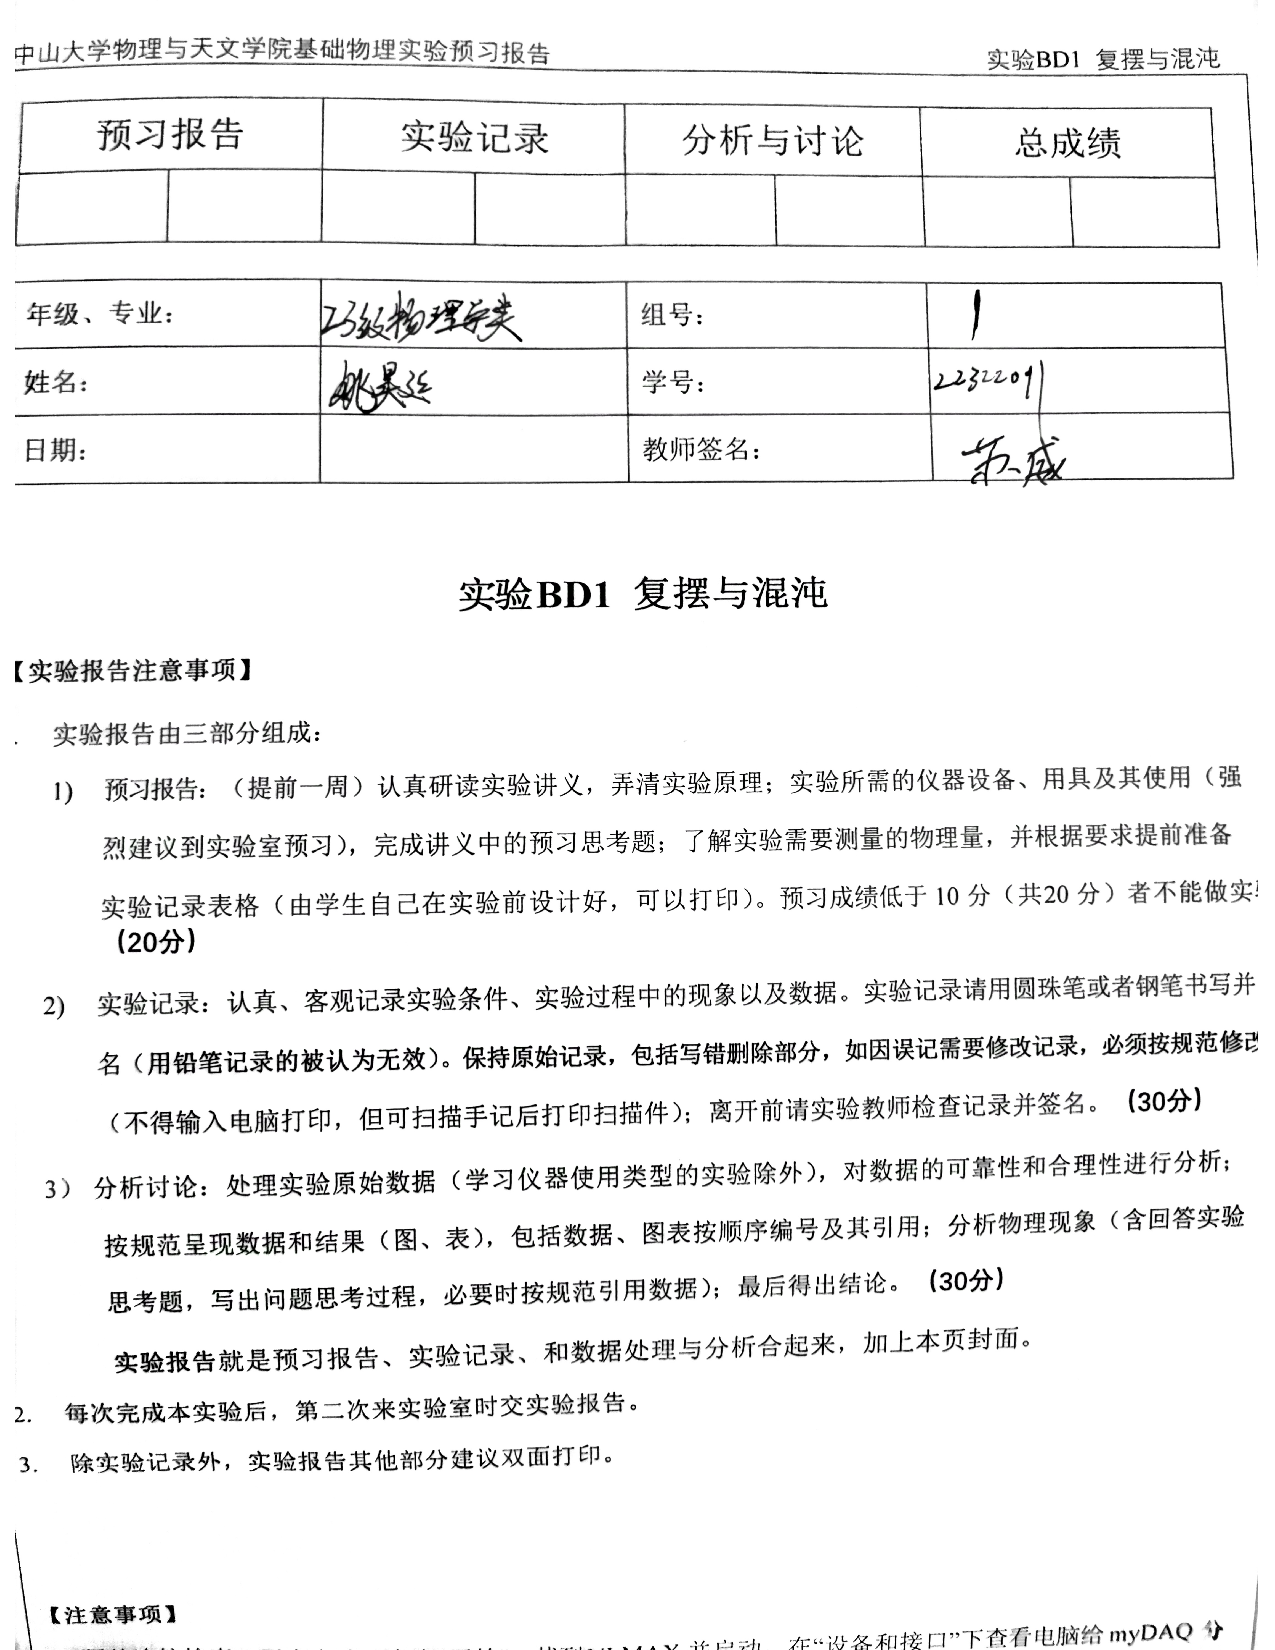
\includepdf[pages=-]{实验3原件.pdf}
%\begin{figure}[H]
%	\centering
%	\includegraphics[width=\textwidth]{焦距数据.jpg}
	
%\end{figure}
%\begin{figure}[H]
%	\centering
%	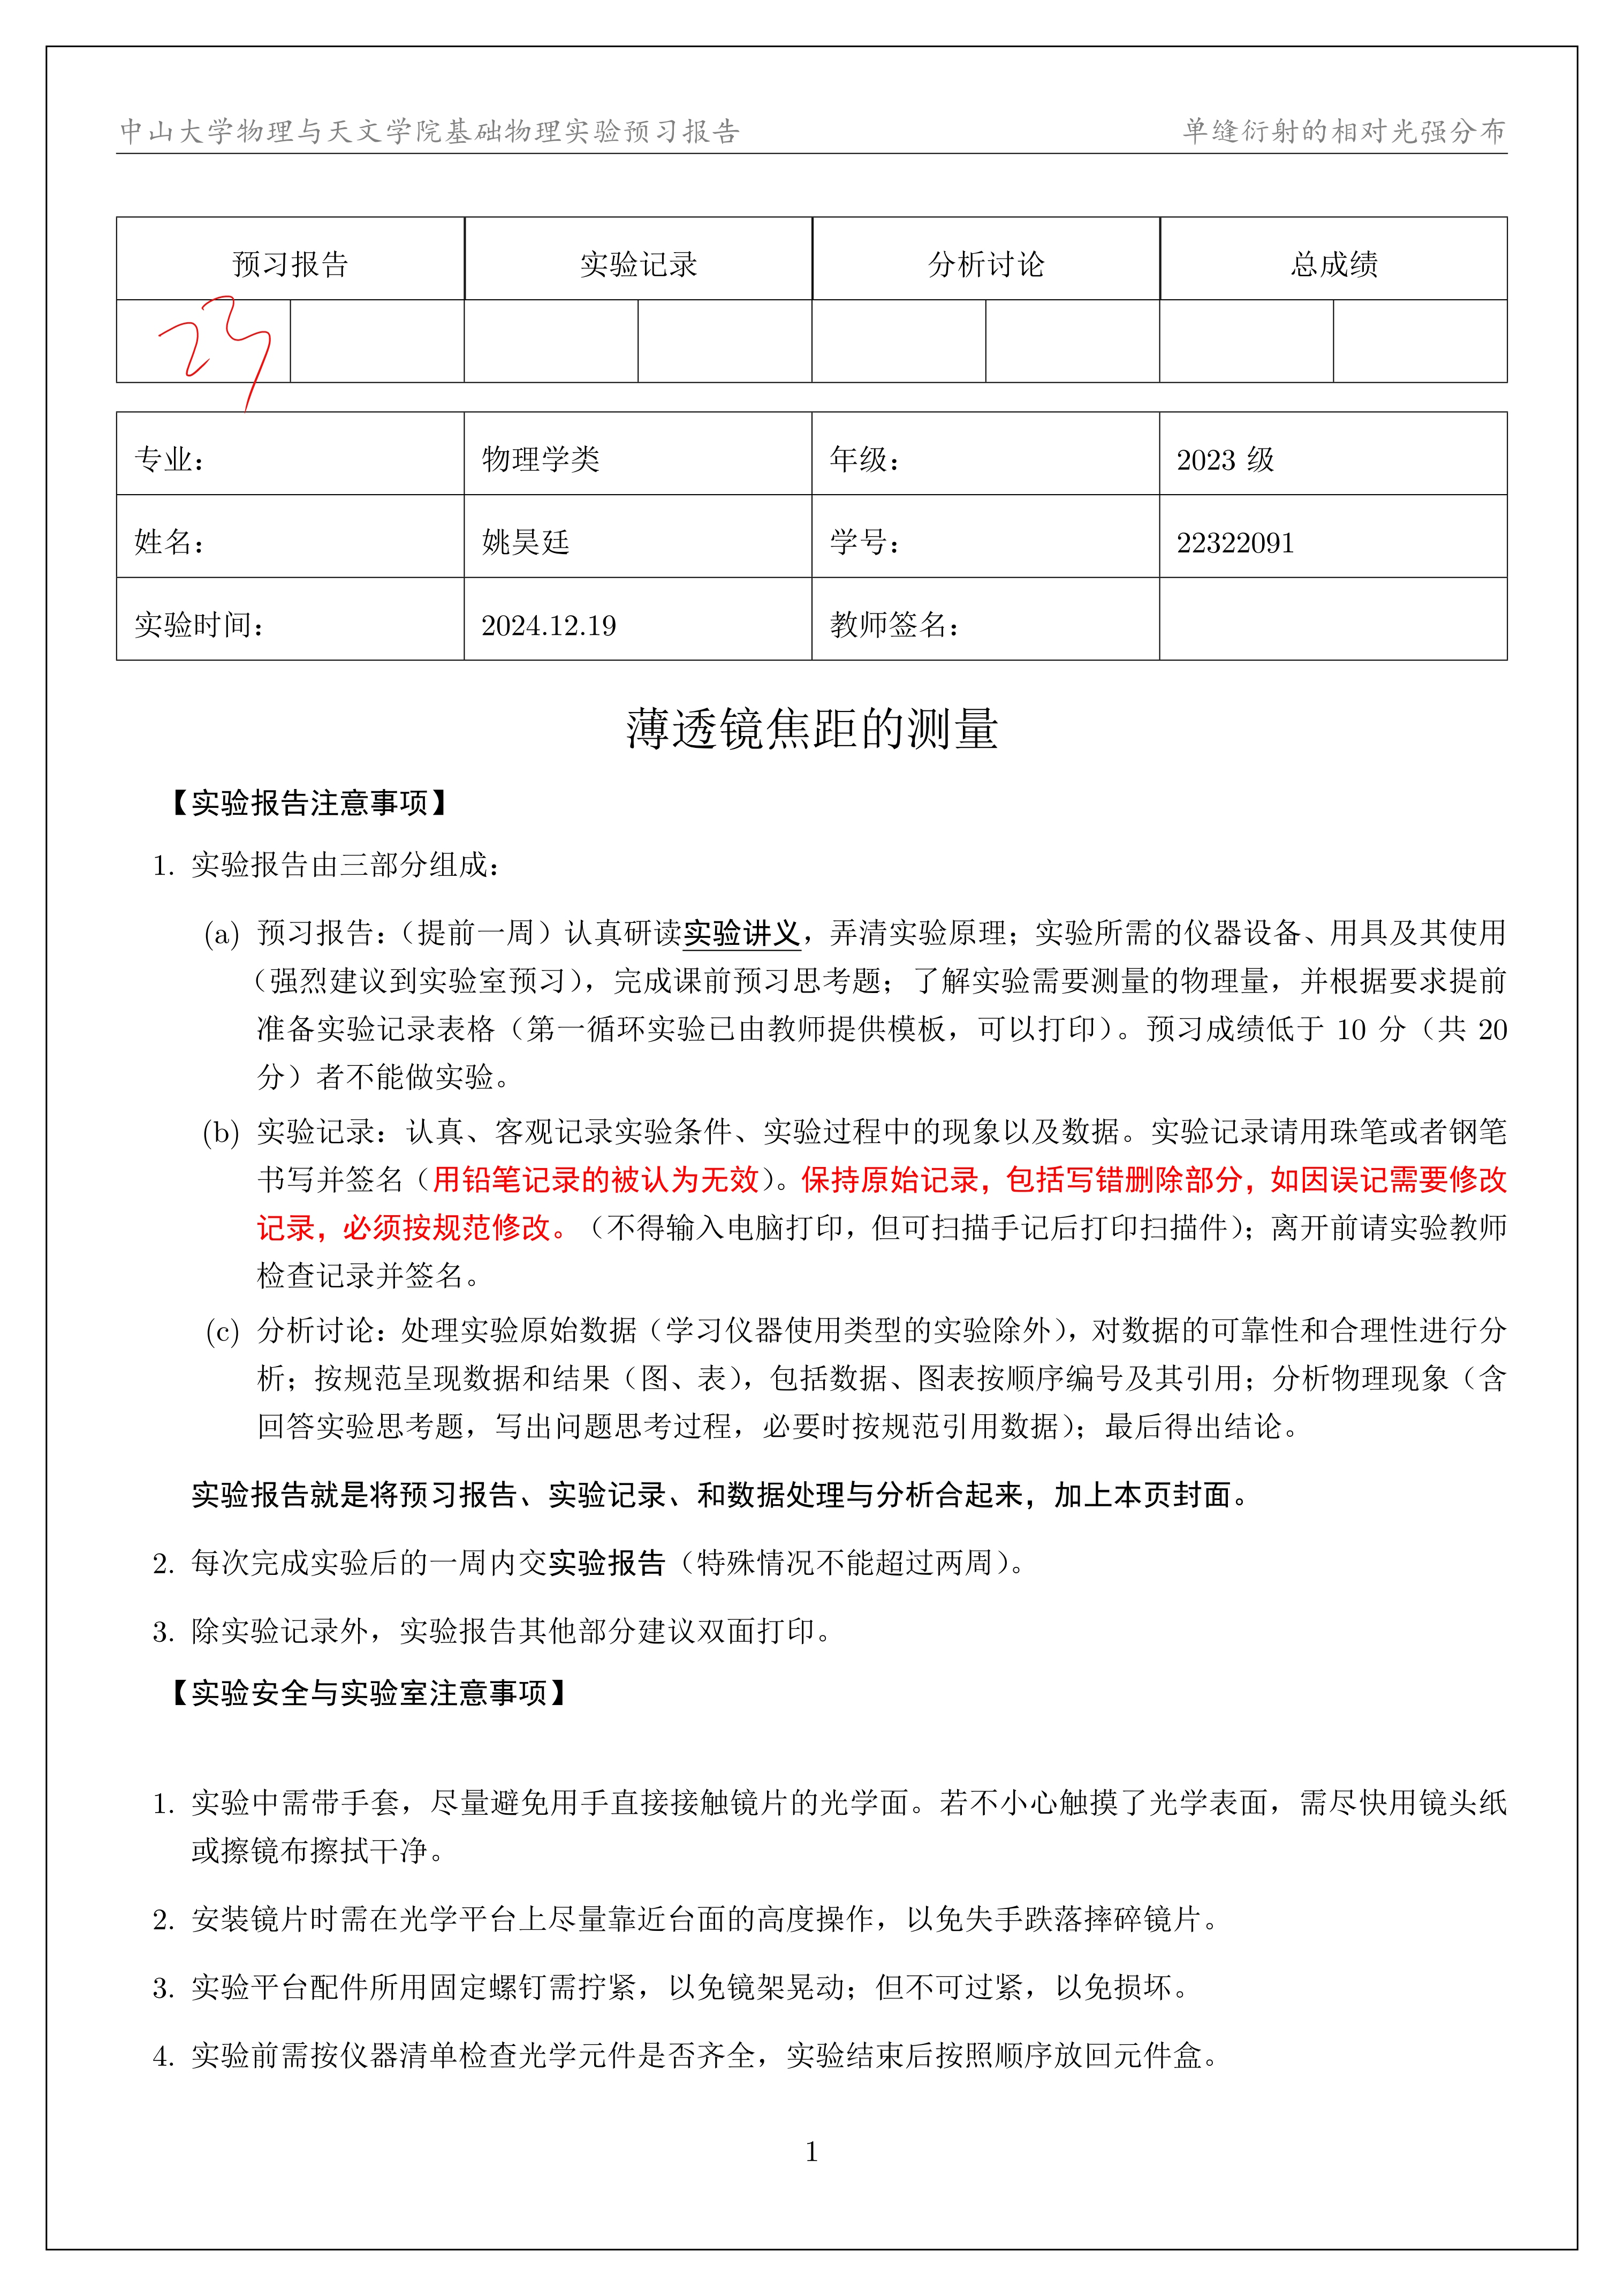
\includegraphics[width=\textwidth]{透镜焦距.jpg}
	
%\end{figure}

%\begin{figure}[H]
%	\centering
%	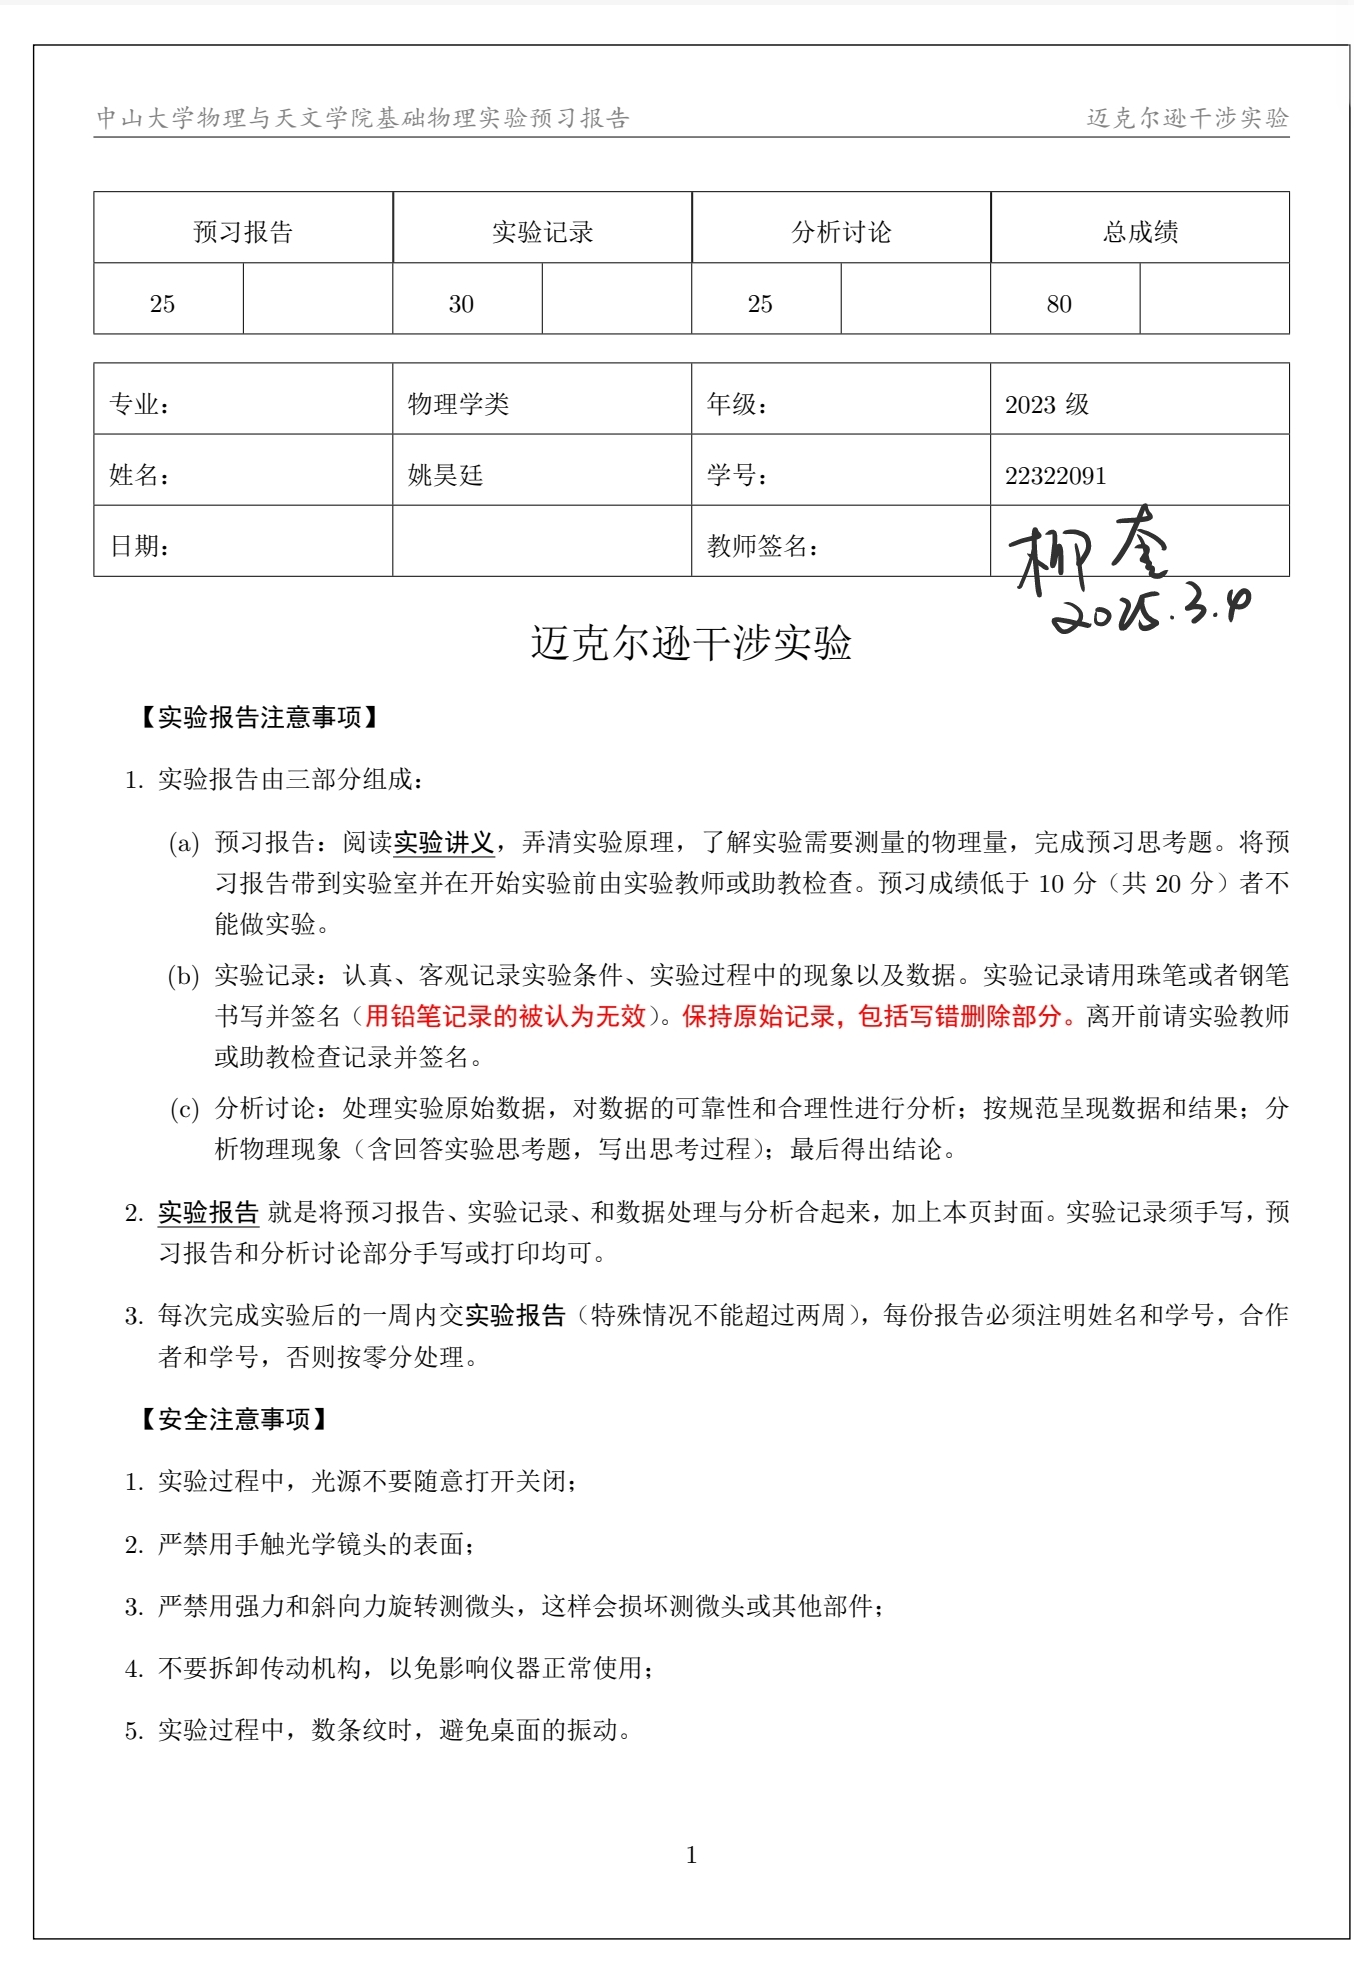
\includegraphics[width=0.4\textwidth]{迈克尔逊原件1.jpg}
%	\includegraphics[width=0.4\textwidth]{迈克尔逊原件2.jpg}
%	\includegraphics[width=0.4\textwidth]{单缝原件3.jpg}
%	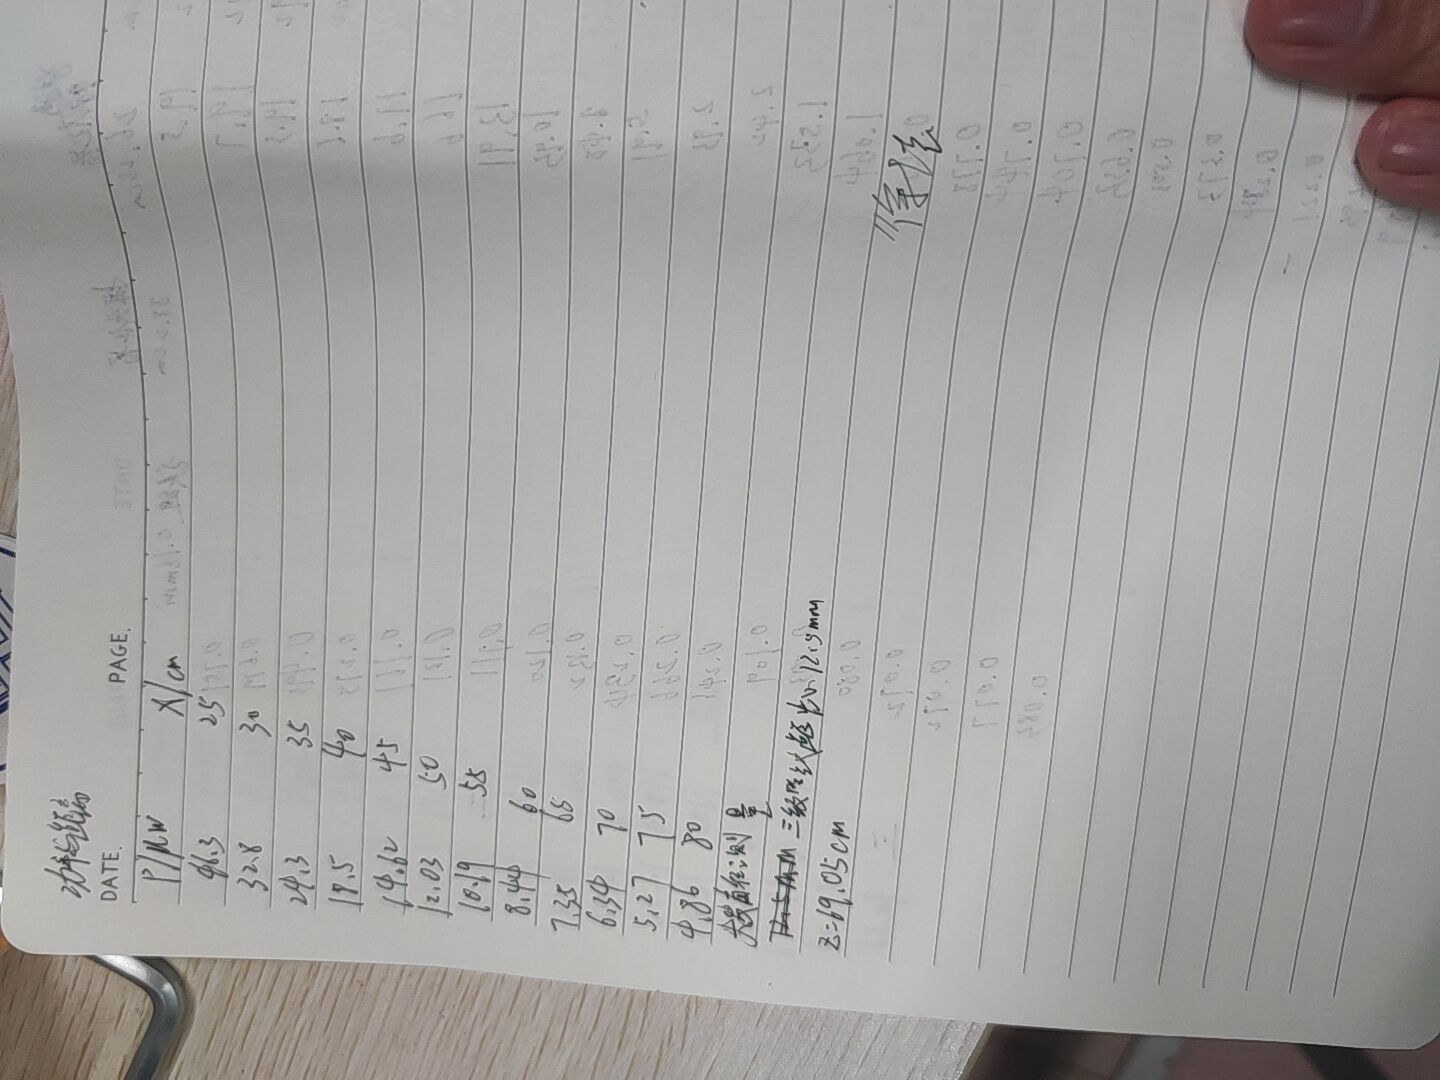
\includegraphics[width=0.4\textwidth]{单缝原件4.jpg}
%\end{figure}
%\subsection*{桌面}
%\begin{figure}[H]
%	\includegraphics[width=0.95\textwidth]{迈克尔逊桌面.jpg}
%\end{figure}
\end{document}
%